\section{Software-Entwicklungsprozess}
Software-Entwicklungsprozesse werden durch sogenannte Vorgehensmodelle strukturiert. Diese Modelle dienen dazu, die Organisation von Software-Entwicklungs\-projekten zu unterstützen, indem sie sämtliche Aktivitäten systematisch in klar definierte und verbindliche Arbeitsschritte gliedern.

Für dieses Projekt wird das Prototyping-Modell eingesetzt. Bei diesem Ansatz werden schrittweise Prototypen basierend auf den aktuellen Anforderungen entwickelt. Das daraufhin eingeholte Feedback von Auftraggebern oder Endanwendern ermöglicht eine kontinuierliche Verfeinerung der Anforderungen und eine schrittweise Verbesserung des Prototyps. Die Stadien dieses Modells werden in Abbildung~\ref{fig:Prototyping-Modell} nochmals verdeutlicht \cite{senarath2021waterfall}.

\begin{figure}[h!]
    \centering
    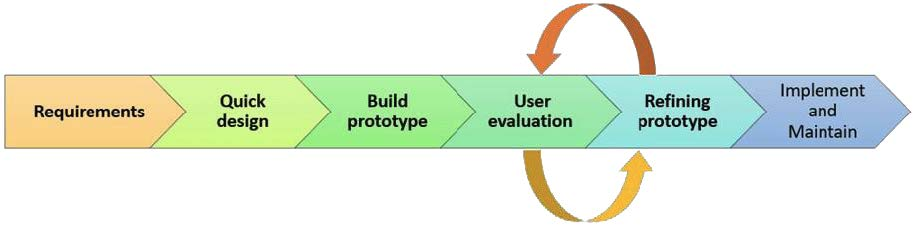
\includegraphics[]{bilder/Prototyping_Stages.jpg}
    \caption{Prototyping-Modell Stadien \cite{senarath2021waterfall}}
    \label{fig:Prototyping-Modell}
\end{figure}


Das Prototyping-Modell wurde eingesetzt, da die Anforderungen des technischen Feasibility Checks zu Beginn noch nicht eindeutig definiert waren und erst im Laufe der Entwicklung bestimmte Aspekte geklärt werden konnten. Außerdem wird das Risiko von Fehl-Entwicklungen minimiert, da der Anwender Ergebnisse schneller evaluieren kann. Zudem fördert dieses Vorgehen den regelmäßigen Austausch zwischen dem Entwickler und den Auftraggebern \cite{senarath2021waterfall}.